In this section, we present our proposed approach to learning inverse dynamics with contacts.
We first formalize the problem as learning a mixture-of-experts model.
Then we detail how we implement Gaussian processes as the corresponding experts.


\subsection{Learning contacts as a mixture-of-experts}
		
		%
	\begin{figure}[t]
		\centering
		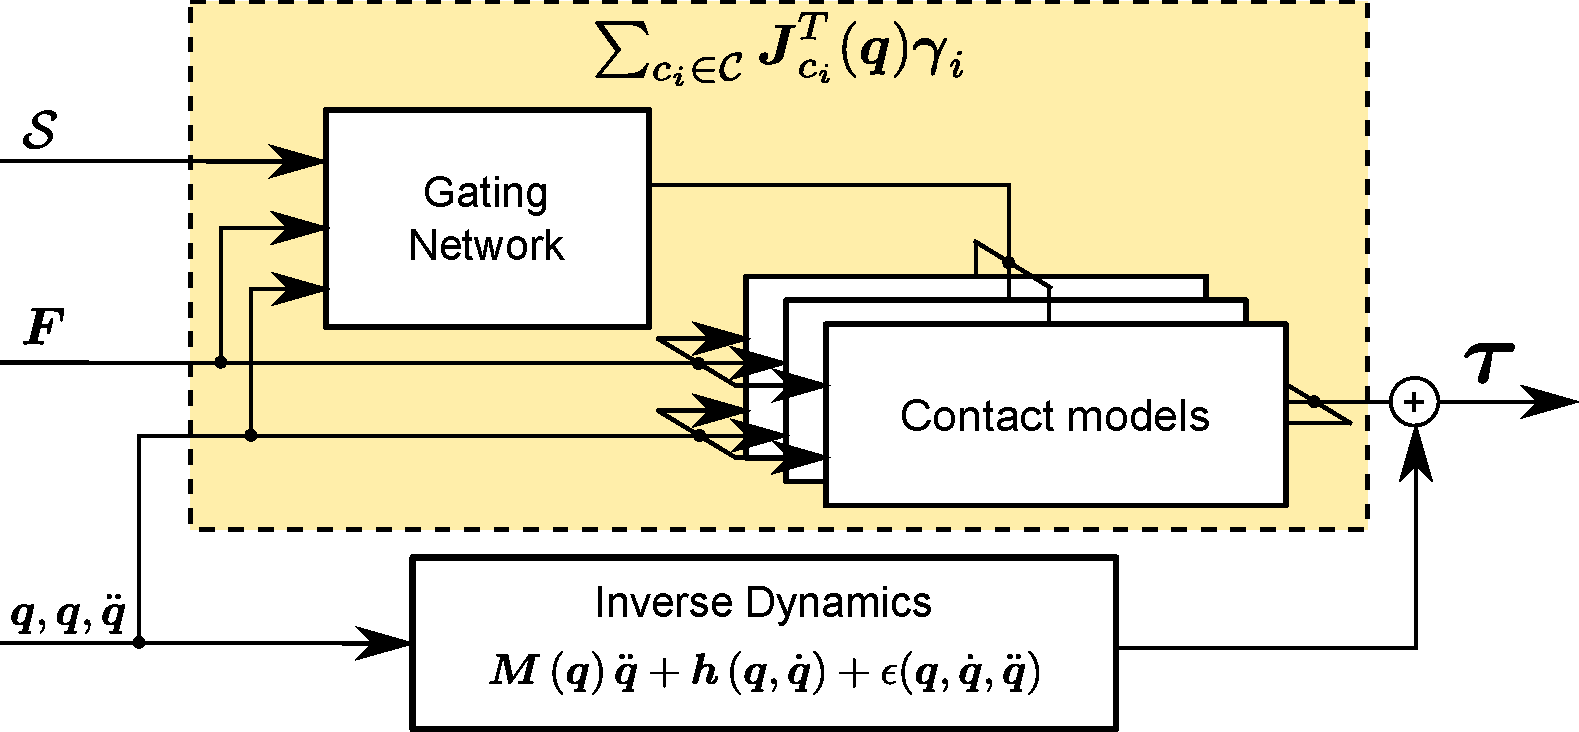
\includegraphics[width =.7\linewidth]{robertoICRA/fig/diagram_2.pdf}
		\caption{Our approach extends existing inverse dynamics without contacts by learning many contact models, which serve as correction terms under different contact types. The decision of which contact model to activate is made by a gating network, which uses skin measurements~$\skinInput$, the force torque sensors~$\ftsForces$ and the current state $\q, \dq, \ddq$.}
		\label{fig:model}
        \figspace
	\end{figure}
	%
	When learning inverse dynamics with contacts \eq\eqref{eq:tau_contact}, we assume that the (contact-free) inverse dynamics from \eq\eqref{eq:tau_nocontact} can be computed precisely, either from an analytical model or from a learned model~\cite{Nguyen-Tuong2011}.
    %
    In our experiments, we employ a learned GP model as contact-free inverse dynamics.
    The reason for this choice are the unmodeled dynamics $\epsilon\,(\q,\dq,\ddq)$, which introduce substantial errors even without contacts.
	%
	As a result of the pre-existing contact-free inverse dynamics, only the model of the residual term of the external forces $\sum_{c_i \in\mathcal{C}} {\jacobian\T_{c_i}(\q)}\, \extForces_i$ has to be separately learned.
    In this paper, we consider a robot that is provided with skin measurements~$\skinInput$ from the tactile sensors, force measurements~$\ftsForces$ from the force torque sensors (FTS) and the ground truth of the torques~$\torques$ from the joint torque sensors (JTS).
    An illustration of these relevant components is shown in \fig\ref{fig:concept}.
	Modeling the external forces $\sum_{c_i \in\mathcal{C}} {\jacobian\T_{c_i}(\q)}\, \extForces_i$ can be formalized as the regression task
  	%
	\begin{align}
		\outputMatrix = \regressionNo([\q, \skinInput]) + \noise\,,
		\label{eq:regression}
	\end{align}
	%    
	where $\outputMatrix = \sum_{c_i \in\mathcal{C}} {\jacobian\T_{c_i}(\q)}\, \extForces_i$ and  
    %$\inputMatrix = [\q, \skinInput,\ftsForces]$ are the inputs. 
	$\noise$ is an i.i.d. Gaussian measurement noise with mean~$0$ and variance~$\sigma_\noise^2$.
% 	Therefore, our regression problem is phrased as
%   	%
% 	\begin{align}
% 		\outputMatrix =\color{darkgreen}{\sum_{i \in\mathcal{C}} {\jacobian_i(\q)}\T \extForces_i} \color{black}{ = \regressionNo([\q, \skinInput,\ftsForces]) + \noise\,.}
% 		\label{eq:regression}
% 	\end{align}
% 	%    
	%
    Contacts with different parts of the body lead to different effects in the dynamics.
    Intuitively, it is necessary to consider the skin input~$\skinInput$ to identify the position of the contact.
	%It is necessary to consider the skin as an input~$\skinInput$ since contacts with different parts of the body lead to different effects in the dynamics.
	%Intuitively, $\skinInput$ is required to identify the position of the contact.
    Additionally, measurements of the force applied by the contacts are necessary to deal with a non-static environment.
    %\todo[inline]{Rephrase sentence above. It's unclear.}
    Theoretically, these measurements can be provided by the skin.
    However, the artificial skin used in our experiments does not provide a precise six-dimensional measure of the contact force.
	Therefore, in the implementation of our model we substitute the force measurement from the skin with the force/torque measurements~$\ftsForces$.
    The corresponding regression problem \eq\eqref{eq:regression} is complicated due to the high-dimensional space of the input $\inputMatrix \in \inputSpace$ (the skin measurements~$\skinInput$ alone account for hundreds of dimensions).
	Therefore, we rephrase this regression task as a problem of learning a mixture-of-experts model.
	With this model, we decompose \eq\eqref{eq:regression} as
	%
	\begin{align}
		\sum\nolimits_{c_i \in\mathcal{C}} {\jacobian\T_{c_i}(\q)}\, \extForces_i \,=\, \sum\nolimits_{j\in\mathcal{J}} f_j([\q, \ftsForces]) + \noise\,,
		\label{eq:expertofmixtureregression}
	\end{align}
	%    
	where $\mathcal{J}$ is the set of active experts~$f_j$.
    %\todo[inline]{What is an active expert? Unclear.}
    %, which depends from $[\q, \skinInput]$.
	Note that the skin input~$\skinInput$ is no longer explicitly part of the inputs of the experts. %\todo{Why?}
    Therefore, each single expert~$f_j$ is now sufficiently low-dimensional to be modeled independently. At the same time the possibility of summing the contribution of each contact allows to account for complex%\todo{I don't like this word} 
    behaviors.
    As single expert~$f_j$ we use Gaussian processes for the mapping $[\q, \ftsForces] \mapsto {\jacobian\T_j(\q)} \extForces_j$.
    %Detailed information regarding the GP models and their training are given in the next subsection.
    A gating network is used to select the experts that are currently active and to add their contributions.    
    An illustration of our approach is shown in \fig\ref{fig:model}.
	%For mixture-of-experts models it is required to design a suitable gating network that activates the relevant experts.
    In this paper, we implement this gating network as a multi-class classifier $\mathcal{J} = g(\q, \skinInput,\ftsForces)$ that selects which contact is currently ongoing.
    %\todo[inline]{In a general setting, the gating network does not make hard decisions. Please make this clear. This would probably also change eq. (4) since you would need weights. }
	For simple tasks, this gating network can be designed using heuristics (e.g., using thresholds on the activation of the tactile sensors). 
    However, for more complex systems an adaptive, data-driven approach may be more suitable. 
    In the experimental section we evaluate the learning of such gating network.
    %\todo[inline]{Strange end of this section. Shall we delete it? It only adds confusion.}
	%This automatic design is increasingly helpful for high number of skin sensor ($>1000$), where the manual design became increasingly complex.

%\todo[inline]{How do you define the experts? And how many do you need? Not mentioned.}

%\todo[inline,color=yellow]{Make sure the section headings are consistently capitalized.}


\subsection{Gaussian processes as expert models}
%\todo[inline]{Introduce GPs only in the context of IDM: distribution over IDMs (instead of "function"), RBD as prior mean, define X and Y in this context immediately.}
	Gaussian Processes (GPs)~\cite{Rasmussen2006} are a state-of-the-art regression method.
	They have been used in robotics to learn dynamics models~\cite{Deisenroth2012} and for control~\cite{Deisenroth2014}.
    %
    In this paper, a GP is a distribution over inverse dynamics models 
	%
	%\begin{align}
		\mbox{$f \sim \GP \left( m_f,k_f \right) \,,$}
	%\end{align}
	%
	fully defined by a prior mean~$m_f$ and a covariance function~$k_f$.
	We choose as prior mean $m_f \equiv \torques_\text{RBD}$ and as covariance function~$k_f$ the squared exponential with automatic relevance determination and Gaussian noise
    %
	\begin{align*}
		{k(\vec x_p,\vec x_q)} &= \sigma_f^2\exp\left(\!-\!\tfrac{1}{2}(\vec x_p\! -\!\vec x_q)^T {\mat \Lambda\inv} (\vec x_p \!-\! \vec x_q)\right) \!+\! \sigma_\noise^2\delta_{pq}
		%\label{sec:GP:cov:SE}
	\end{align*}
	%
	where ${\mat \Lambda}=\diag([l^2_1,...,l^2_D])$ and $\delta_{pq}$ is the Kronecker delta (which is one if $p=q$ and zero otherwise). Here, $l_i$ are the length-scales, $\sigma^2_f$ is the variance of the latent function $f(\cdot)$ and $\sigma^2_\noise$ the noise variance. 
 %   The purpose of $\sigma_w^2\delta_{pq}$ is to model (and identify) the presence of the Gaussian noise~$\epsilon$.
 
    In our experiments, when learning contact models, the input is defined as $\parameters = [\q,\ftsForces]$, while the output (observations) $\vec y = \torques$ are the torques.
    Hence, given $n$ training inputs $\mat X=[\parameters_1,...,\parameters_n]$ and corresponding training targets $\mat y=[ y_1,..., y_n]$, we define the training data set $\dataset = \{\mat X,\mat y\}$. 
    % training
Training the GP corresponds to finding good hyperparameters $\vec \theta = [l_i, \sigma_f, \sigma_\noise]$, which is done by the standard procedure of maximizing the marginal likelihood~\cite{Rasmussen2006}.   
    
% predictive distribution    
    The GP yields the predictive distribution over torques for a new input $\vec x_* = [\vec q_*, \mat F_*]$
	%
	\begin{align}
		&\prob(\vec y|\dataset,\parameters_*,\vec \theta) = \gauss{\mu(\parameters_*)}{\sigma^2(\parameters_*)}\,, 
		\label{eq:one-step prediction distr}
	\end{align}
	%
	where the mean~$\mu(\parameters_*)$ and the variance~$\sigma^2(\parameters_*)$ are 
	%
	\begin{align}
		&\mu(\parameters_*) = \vec k^T_*\vec K^{-1} \mat y\,,\quad \sigma^2(\parameters_*) = k_{**}-\vec k^T_*\mat K^{-1}\vec k_*\,,
		\label{eq:one-step prediction mean and covariance}
		%\label{eq:one-step prediction cov}
	\end{align}
	%
	%% all the stuff from the equations
    respectively.	The entries of the matrix $\vec K$ are  $K_{ij}= k(\parameters_i,\parameters_j)$, and we define $k_{**}=k(\parameters,\parameters)$ and $\vec k_{*}=k(\vec X,\parameters)$.
    
    %\todo[inline]{It remains unclear how you use the GPs as experts in the MoE model. How do you determine the corresponding training data sets? What is the number of experts? And you also need to explain the gating network much better.}